\documentclass[../main/main.tex]{subfiles}

\raggedbottom

\makeatletter
\renewcommand{\@chapapp}{\'Electrocin\'etique -- chapitre}
\makeatother

\begin{document}
\setcounter{chapter}{1}

\chapter{R\'esistances et sources}

\section{Généralité sur les dipôles}
\subsection{Caractéristique d'un dipôle}
\begin{tcbraster}[raster columns=2, raster equal height=rows]
    \begin{defi}[label=def:dipcara]{Caractéristique}

        On appelle \textbf{caractéristique} d'un dipôle la fonction $I = f(U)$
        (ou $U = g(I)$ selon la convention). Sauf indication contraire, elle est
        déterminée \textbf{en régime continu}.

        \tcbsubtitle[before skip=\baselineskip,
        colback=green!50!black,
        colframe=green!50!black]{Cas particuliers}

        Un dipôle en \textbf{court-circuit} (branchement d'un fil aux bornes) a
        pour tension $U = 0$, et ce pour tout $I$. Un dipôle qui n'est
        \textbf{pas relié à un circuit fermé} a pour intensité $I = 0$.
    \end{defi}
    \begin{exem}[label=exem:dipcara]{Exemple}
        \begin{center}
            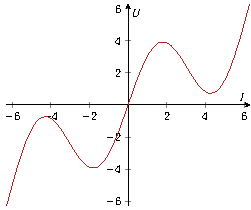
\includegraphics[width=\linewidth]{carac_gen}
        \end{center}
    \end{exem}
\end{tcbraster}

\subsection{Classification de dipôles}
\begin{defi}[label=def:actifpassif]{{Actif ou passif, linéaire ou non,
    symétrique ou non}}

    \begin{defiside}
        
        On appelle \textbf{passif} un dipôle qui reçoit \textbf{toute son
        énergie} du circuit, il n'est \textbf{pas} alimenté par une
        \textbf{source extérieure}. C'est équivalent à dire que \fbox{\textbf{sa
        caractéristique passe par (0,0)}}. On utilise pour eux la convention
        \textbf{récepteur}.

    \tcblower

        On appelle \textbf{actif} un dipôle qui reçoit de l'énergie de
        l'extérieur du circuit, \textit{via} une \textbf{alimentation externe}.
        C'est équivalent à dire que \fbox{\textbf{sa caractéristique NE passe
        PAS par 0}}. On utilise pour eux la convention \textbf{générateur}.
    \end{defiside}
    \hrule
    \begin{defiside}
        Un dipôle est dit \textbf{linéaire} si sa caractéristique est une
        \textbf{droite}.

        \tcblower

        Un dipôle est dit \textbf{non-linéaire} si sa caractéristique n'est
        \textbf{pas une droite}.
    \end{defiside}
    \hrule
    \begin{defiside}
        Un dipôle est dit \textbf{symétrique} si sa caractéristique est
        \textbf{impaire}. \fbox{Un dipôle symétrique est forcément passif}.

        \tcblower

        Un dipôle est dit \textbf{asymétrique} si sa caractéristique est
        \textbf{paire}.
    \end{defiside}
\end{defi}

\section{Résistance}
\subsection{Définition et schéma}

Lorsqu'un courant circule dans un matériau conducteur, les électrons sont
freinés par les atomes de celui-ci. Cet effet est maximal dans certains dipôles
que l'on appellera des conducteurs ohmiques ou résistors. Par abus de langage,
on désignera le composant par le même nom que la grandeur physique qui le
caractérise~: la résistance.

\begin{tcbraster}[raster columns=3, raster equal height=rows]
    \begin{defi}[label=def:resistance]{résistance}
        Une résistance est un dipôle \textbf{récepteur}, dont la caractéristique en
        convention récepteur suit la \textbf{loi d'Ohm}~:
        \[\boxed{U=RI}\]
        avec $R$ la valeur de la résistance en Ohm ($\Omega$) telle que $R > 0$. On
        définit également la \textbf{conductance} \fbox{$G=1/R$} en Siemens (S).
    \end{defi}
    \begin{impl}[label=impl:resistance]{puissance}
        En utilisant la caractéristique de la résistance et l'expression de la
        puissance d'un dipôle, on a
        \[ \boxed{P_{\text{reçue}} = RI^2 = \frac{U^2}{R} = GU^2}\]
        Qui est positive. Dans le cas de la résistance, cette puissance est
        entièrement \textbf{dissipée} par effet \textsc{Joule}.
    \end{impl}
    \begin{exem}[label=exem:resistance]{schémas}
        \begin{center}
            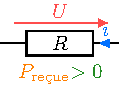
\includegraphics[width=\linewidth]{resistance}
            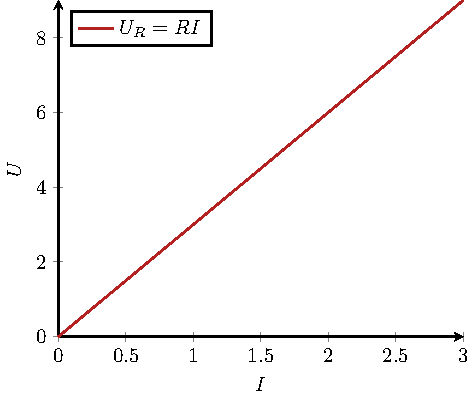
\includegraphics[width=\linewidth]{carac_R}
        \end{center}
    \end{exem}
\end{tcbraster}

\subsection{Association de résistances en série}
\begin{tcbraster}[raster columns=2, raster equal height=rows]
    \begin{prop}[label=prop:rserie]{association en série}
        Deux résistances $R_1$ et $R_2$ en série forment un dipôle équivalent de
        résistance
        \[\boxed{R_{\rm eq} = R_1 + R_2}\]
        On dit qu'\textbf{en série, les résistances s'ajoutent}.
        \tcblower
        \begin{center}
            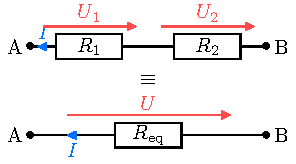
\includegraphics[width=\linewidth]{rserie}
        \end{center}
    \end{prop}
    \begin{demo}[label=demo:rserie]{association en série}
        À partir du schéma précédent, on écrit la loi d'additivité des tensions,
        puis on applique la loi d'Ohm et on factorise~:
        \begin{align*}
            U &= U_1 + U_2\\
            U &= R_1I + R_2I\\
            U &= (R_1 + R_2)I
        \end{align*}
        On a bien l'expression d'un unique conducteur ohmique de résistance
        \fbox{$R_{\rm eq} = R_1 + R_2$}.
    \end{demo}
\end{tcbraster}

\subsection{Association de résistances en parallèle}
\begin{tcbraster}[raster columns=2, raster equal height=rows]
    \begin{prop}[label=prop:rpara]{association en parallèle}
        Deux résistances $R_1$ et $R_2$ en dérivation forment un dipôle
        équivalent de résistance
        \[ \boxed{\dfrac{1}{R_{\rm eq}} = \dfrac{1}{R_1} + \dfrac{1}{R_2}}
        \Longleftrightarrow \boxed{R_{\rm eq} = \frac{R_1R_2}{R_1 + R_2}}\]
        On dit qu'\textbf{en parallèle, l'inverse des résistances s'ajoutent}.
        \tcblower
        \begin{center}
            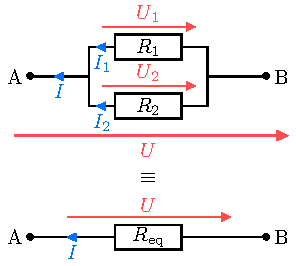
\includegraphics[width=\linewidth]{rpara}
        \end{center}
    \end{prop}
    \begin{demo}[label=demo:rpara]{association en parallèle}
        On applique la loi des nœuds~: \[I = I_1+I_2\]
        On utilise ensuite la loi d'Ohm~:
        \[I = \frac{U}{R_1} + \frac{U}{R_2}\]

        On trouve $R_{\rm eq}$ en exprimant la caractéristique du dipôle
        équivalent sous la forme $I = G_{\rm eq}U$, puis $G_{\rm eq} = 1/R_{\rm
        eq}$, d'où ici

        \[I = \left(\dfrac{1}{R_1} + \dfrac{1}{R_2}\right) U\]
        On a bien l'expression d'un unique conducteur ohmique de résistance
        \[\boxed{\dfrac{1}{R_{\rm eq}} = \dfrac{1}{R_1} + \dfrac{1}{R_2}}
        \Longleftrightarrow \boxed{R_{\rm eq} = \frac{R_1R_2}{R_1 + R_2}}\]
    \end{demo}
\end{tcbraster}
\begin{NCexem}[sidebyside]{Exercice d'application}

    Exprimer en fonction de $R$ la résistance équivalente entre A et B pour
    l'association ci-dessous.
    \begin{center}
        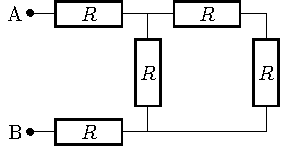
\includegraphics[width=\linewidth]{exer_rasso-plain}
    \end{center}
    \tcblower
    \begin{center}
        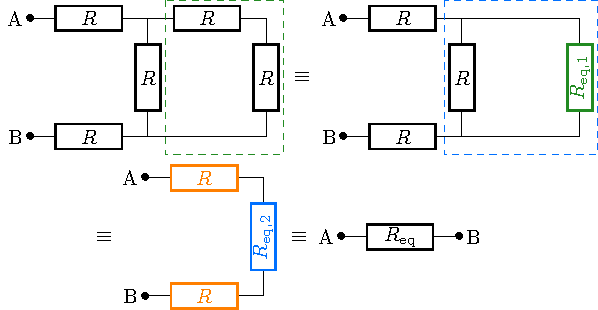
\includegraphics[width=\linewidth]{exer_rasso}
    \end{center}
    \begin{align*}
        R_{\rm eq}                 & = \textcolor{orange}{R + R} +
            \textcolor{brandeisblue}{R_{\rm eq,2}} \\
        \Leftrightarrow R_{\rm eq} & = \textcolor{orange}{2R} +
            \textcolor{brandeisblue}{\frac{
                    R\times \textcolor{ForestGreen}{R_{\rm eq,1}}
            }{R + \textcolor{ForestGreen}{R_{\rm eq,1}}}}\\
        \Leftrightarrow R_{\rm eq} & = 2R + \frac{
            R\times\textcolor{ForestGreen}{2R}}{
            R+\textcolor{ForestGreen}{2R}} \\
        \Leftrightarrow R_{\rm eq} & = 2R + \frac{2R^{\cancel{2}}}{3\cancel{R}}\\
        \Leftrightarrow R_{\rm eq} & = \frac{8R}{3}
    \end{align*}
\end{NCexem}

\subsection{Les ponts diviseurs}

Les ponts diviseurs sont des relations permettant de trouver des courants ou des
tensions dans certains cas particuliers, sans repasser par l'écriture des lois
des nœuds, des mailles et d'Ohm.

\subsubsection{Pont diviseur de tension}

\begin{tcbraster}[raster columns=2, raster equal height=rows]
    \begin{prop}[label=prop:divtens, sidebyside]{pont diviseur de tension}
        Soit le circuit ci-après, où $U$, $R_1$ et $R_2$ sont connus et on
        cherche $U_1$ ou $U_2$. Dans ces conditions, on a
        \[ \boxed{U_k = \frac{R_k}{R_1+R_2}U_{AC}}\]
        qui se généralise en
        \[ \boxed{U_k = \frac{R_k}{R_{\rm eq}}U}\]
        \tcblower
        \begin{center}
            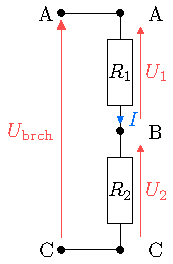
\includegraphics[width=\linewidth]{divis_tension}
        \end{center}
    \end{prop}
    \begin{demo}[label=demo:divtens]{pont diviseur de tension}
        Avec une loi des mailles et la loi d'Ohm pour les résistances, on trouve
        \[ I = \frac{U_{AC}}{R_1+R_2}\]
        En réappliquant la loi d'Ohm pour $R_2$ par exemple, on trouve
        \[ U_{AB} = R_2I = \frac{R_2}{R_1+R_2}U_{AC} \]
        Le calcul est tout à fait similaire pour le cas avec plus de résistances
        dans la branche.
    \end{demo}
\end{tcbraster}

\subsubsection{Pont diviseur de courant}

\begin{tcbraster}[raster columns=2, raster equal height=rows]
    \begin{prop}[label=prop:divcour]{pont diviseur de courant}
        Soit le circuit ci-après, où $I$, $R_1$ et $R_2$ sont connus et on
        cherche $I_1$ ou $I_2$. Dans ces conditions, on a
        \[ \boxed{I_{\fbox{2}} = \frac{R_{\fbox{1}}}{R_1+R_2}I}
        \Longleftrightarrow \boxed{I_k = \frac{G_k}{G_1+G_2}I}\]
        Avec $R_{\rm eq}$ la résistance équivalente entre $A$ et $B$, ceci se
        généralise en
        \[ \boxed{I_k = \frac{R_{\rm eq}}{R_k}I}
        \Longleftrightarrow \boxed{I_k = \frac{G_k}{G_{\rm eq}}I}\]
        \tcblower
        \begin{center}
            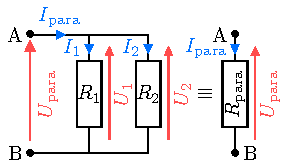
\includegraphics[width=.6\linewidth]{divis_courant}
        \end{center}
    \end{prop}
    \begin{demo}[label=demo:divcour]{pont diviseur de courant}
        Avec la loi des nœuds, on a
        \[I = I_1 + I_2\]
        Avec la loi d'Ohm pour les résistances et par égalité des tensions dû au
        montage parallèle, on a
        \[I = \frac{U}{R_1} + \frac{U}{R_2} = \frac{U}{R_{\rm eq}} = G_{\rm eq}U\]
        D'où, pour $I_1$ par exemple,
        \[I_1 = \frac{U}{R_1} = \frac{R_{\rm eq}}{R_1}I\]
        ou
        \[I_1 = G_1 U = \frac{G_1}{G_{\rm eq}}I\]

        Le calcul est tout à fait similaire pour le cas avec plus de résistances
        en parallèle.
    \end{demo}
\end{tcbraster}

\subsubsection{Attention}
\begin{ror}[label=impo:ponts]{utilisation des ponts}

    \textbf{Attention} aux conditions d'application de ces formules. Notamment,
    les résistances \textbf{doivent être en série} pour le pont diviseur de
    \textbf{tension}, et en \textbf{parallèle} pour le pont diviseur de
    \textbf{courant}. Si ça n'est pas le cas, simplifier le circuit pour se
    ramener à cette forme. De plus, il faut vérifier \textbf{le sens
    d'orientation des tensions et intensités}. Autrement dit, connaissez bien
    votre cours pour le reproduire exactement puis adaptez les notations à celle
    de l'exercice.
    
\end{ror}

\section{Sources}
\subsection{Source idéale de tension}

\begin{tcbraster}[raster columns=2, raster equal height=rows]
    \begin{defi}[label=def:gentens]{générateur idéal de tension}

        Un générateur de tension est alimenté par une source d'énergie
        extérieure au circuit et \textbf{impose une tension}, le courant débité
        est lui imposé par le reste du circuit électrique.

        \tcblower

        Il est dit \textbf{idéal} si la tension imposée est constante quel que
        soit le courant débité.
    \end{defi}
    \begin{exem}[label=exem:gentens, sidebyside, righthand width=.25\linewidth]
        {schémas}
        \begin{center}
            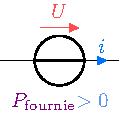
\includegraphics[width=\linewidth]{gconvg}
        \end{center}
        \tcblower
        \begin{center}
            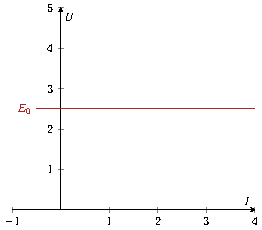
\includegraphics[width=\linewidth]{carac_tens}
        \end{center}
    \end{exem}
\end{tcbraster}

\vspace{-15pt}
\subsection{Source réelle de tension}
\begin{tcbraster}[raster columns=3, raster equal height=rows]
    \begin{defi}[label=def:gentens, sidebyside, raster multicolumn=2]
        {générateur idéal de tension}

        Dans un générateur réel, il y a toujours des effets résistifs qui font
        que la tension imposée et le courant débité sont liés. On a alors
        \[\boxed{U = E_0 - ri}\]
        \tcblower
        Cette modélisation est celle du \textbf{générateur de Thévenin}, et
        $E_0$ est la \textbf{force électromotrice}.

    \end{defi}
    \begin{exem}[label=exem:gentens, sidebyside, righthand ratio=0.7]{schémas}
        \begin{center}
            \rotatebox{90}{
            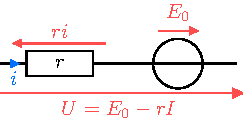
\includegraphics[scale=.8]{thevenin}
        }
        \end{center}
        \tcblower
        \begin{center}
            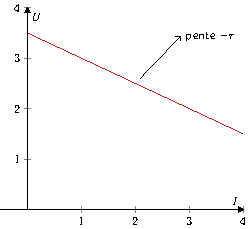
\includegraphics[width=\linewidth]{carac_thev}
        \end{center}
    \end{exem}
\end{tcbraster}

\vspace{-15pt}
\subsection{Résistance de sortie}

\begin{tcbraster}[raster columns=2, raster equal height=rows]
    \begin{prop}[label=prop:rsortie, sidebyside]{résistance de sortie}
        Un générateur réel de force électromotrice $E_0$ et de résistance
        interne $r$ alimentant une résistance R se comporte comme un générateur
        idéal si
        \[ \boxed{R \gg r}\]
        \tcblower
        \begin{center}
            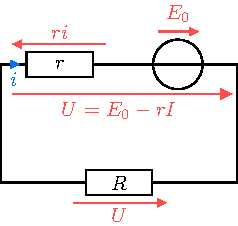
\includegraphics[width=\linewidth]{rsortie}
        \end{center}
    \end{prop}
    \begin{demo}[label=demo:rsortie]{résistance de sortie}
        On applique la formule du pont diviseur de tension pour avoir la tension
        $U$~:
        \[ U = \frac{R}{R + r}E_0\]
        Si on a bien $U \neq E_0$, si $R \gg r$ on a tout de même $U \approx
        E_0$.
    \end{demo}
\end{tcbraster}

\subsection{Source idéale de courant}

\begin{tcbraster}[raster columns=2, raster equal height=rows]
    \begin{defi}[label=def:gentens]{générateur idéal de tension}

        Un générateur de courant est alimenté par une source d'énergie
        extérieure au circuit et \textbf{impose un courant}. La tension a ses
        bornes lui est imposée par le reste du circuit électrique.

        \tcblower

        Il est dit \textbf{idéal} si le courant débité est constante quelle que
        soit la tension à ses bornes.
    \end{defi}
    \begin{exem}[label=exem:gentens, sidebyside, righthand width=.25\linewidth]
        {schémas}
        \begin{center}
            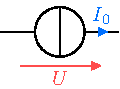
\includegraphics[width=\linewidth]{gcourg}
        \end{center}
        \tcblower
        \begin{center}
            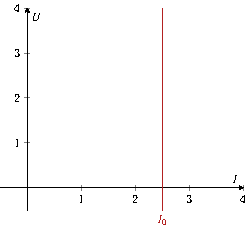
\includegraphics[width=\linewidth]{carac_cour}
        \end{center}
    \end{exem}
\end{tcbraster}

\subsection{Complément~: source réelle de courant}
\begin{tcbraster}[raster columns=2, raster equal height=rows]
    \begin{defi}[label=def:gencour]{générateur idéal de courant}

        Dans un générateur réel, il y a toujours des effets résistifs qui font
        que la tension imposée et le courant débité sont liés. On modélise un
        tel générateur de courant par le \textbf{générateur de Norton}.

    \end{defi}
    \begin{exem}[label=exem:gentens]{schéma}
        \begin{center}
            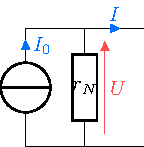
\includegraphics[width=.5\linewidth]{norton}
        \end{center}
    \end{exem}
\end{tcbraster}

\subsection{Résistance de sortie}

\begin{tcbraster}[raster columns=2, raster equal height=rows]
    \begin{prop}[label=prop:rsortie, sidebyside]{résistance de sortie}
        Un générateur d'intensité réel d'intensité $I$ et de résistance
        interne $r_N$ alimentant une résistance R se comporte comme un générateur
        idéal si
        \[ \boxed{R \ll r_N}\]
        \tcblower
        \begin{center}
            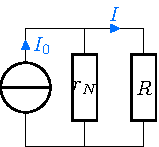
\includegraphics[width=\linewidth]{rsortie_intens}
        \end{center}
    \end{prop}
    \begin{demo}[label=demo:rsortie]{résistance de sortie}
        On applique la formule du pont diviseur de courant pour avoir le courant
        $i$~:
        \[ i = \frac{r_N}{r_N + R}I\]
        Si on a bien $i \neq I$, si $R \ll r_N$ on a tout de même $i \approx
        I$.
    \end{demo}
\end{tcbraster}

\end{document}
